% !TEX root = ../main.tex

% 预习报告	
\setcounter{section}{0}
\section{测量放大器 \\ Preview Report}


%---------------------------------------------------------------------
% 实验目的
\subsection{Purpose}
\begin{enumerate}
	\item 深入了解差分电路的原理,以及其关键参数:共模抑制比(CMRR)、输入电阻、输入及输出电压范围(非失真放大的范围)、放大倍数以及频率响应。
	\item 掌握差分探测在实际测量中的应用。
	\item 熟悉模拟电路仿真套件的使用。
\end{enumerate}


%---------------------------------------------------------------------
% 仪器用具
\subsection{Instruments \& Equipment}
\begin{table}[htbp]
	\centering
	\renewcommand\arraystretch{1.6}
	% \setlength{\tabcolsep}{10mm}
	\begin{tabular}{|p{0.08\textwidth}|p{0.2\textwidth}|p{0.08\textwidth}|p{0.5\textwidth}|}
		\hline
		Number & Name & Quantity & Main parameters (model, measurement range, measurement accuracy, etc.) \\
		\hline
		1 & 函数信号发生器 & 1 & DG4152 \\

		2 & 示波器 & 1 & DS1104 \\

		3 & 直流稳压电源 & 1 & DP832 \\

		4 & 导线 & 若干 &  \\

		5 & $Model_A$ 电路模块 & 若干 & 同相放大器、反相放大器 \\

		6 & $Model_D$ 电路模块 & 若干 &  差分放大、仪表放大 \\

		7 & $Model_E$ 电路模块 & 若干 & INA114 仪表放大器 \\

		8 & 主板电路模块 &  &  \\
		\hline
	\end{tabular}
\end{table}


%---------------------------------------------------------------------
% 原理概述
\clearpage
\subsection{Principle}

	\begin{itemize}
		\item 差模信号与共模信号:

			差模信号是指在两个导线之间传输的信号,其在两个导线上的电压是相反的。也就是说,如果一个导线上的电压是V,那么另一个导线上的电压就是 −V。

			共模信号是指在两个导线之间传输的信号,其在两个导线上的电压是相同的。也就是说,如果一个导上的电压是 V,那么另一个导线上的电压也是V。

			差模信号有很强的靠干扰能力。由于差模信号在两个导线上的电压是相反的,因此当外部噪声同时作用在两个导线上时,这些噪声会被抵消掉,从而提高了信号的抗干扰能力。

			在实际的信号传输中,信号往往是由差模信号和共模信号的叠加组成的。为了提高信号的传输质量和抗干扰能力,通常需要采取一些措施来抑制共模信号的影响,比如使用差分放大器,即我们本实验的出发点之一。

		\item 共模抑制比:
			
			共模抑制比是衡量差分放大器性能的一个重要指标,它表示放大器对差模信号的增益与对共模信号的增益之比,其定义为放大器对差模信号的电压放大倍数 $A_{ud}$ 与对共模信号的电压放大倍数 $A_{uc}$之比。
			\[
				CMRR = \frac{A_{ud}}{A_{uc}}
			\]

			其通常也以分贝(dB)为单位表示:
			\[
				CMRR(\text{dB}) = 20 \log\frac{A_{ud}}{A_{cd}}
			\]

			共模抑制比衡量了放大器在放大差模信号的同时,对共模信号的抑制能力。高CMRR意味着放大器能够更好地抑制共模干扰,从而保持信号的完整性,确保信号在传输过程中能够准确地保持其原始特征。


		\item 基本设计思路:
			\begin{enumerate}
				\item \textbf{先放大后差分:}
				
					考虑先将两路信号分别进行同等倍数的放大,然后进行差分处理。

					现有的Model——E模块可以实现仪表放大器的功能,即“先放大后差分”。

					
				\item \textbf{先差分后放大:}
				
					考虑先将两路信号进行差分,然后进行放大处理。

					考虑将现有的Model——D 和 Model——A 串联使用。

					\begin{itemize}
						\item Model——D 使用方法:
							
							跳线JP1 连接2,3,跳线JP2 连接2,3,并使用3个OP07芯片,即可实现差分放大器的功能,其增益固定为10倍。

						\item Model——A 使用方法:
						
							做同相放大器时:跳线JP1 连接1,2,跳线JP2 断开,跳线JP3 闭合,跳线JP4 闭合以保证增益可调。

							做反相放大器时:跳线JP1 连接2,3,跳线JP2 断开,跳线JP3 断开,跳线JP4 闭合以保证增益可调。
					\end{itemize}
			\end{enumerate}


		\item -3dB 频率的含义
			
			在声学和电子学中,-3dB 频率(也称为截止频率)是一个特定的频率点,用来描述一个滤波器或系统对信号的增益或衰减。dB是分贝(decibel)的缩写,是一个对数单位,用来表示两个物理量(如功率、强度或电压)的比值。

			具体来说,-3dB 频率是指在滤波器或系统的频率响应曲线上,增益或衰减达到-3分贝的频率点。由于分贝是一个对数单位,-3dB 表示功率比(或信号强度比)下降到了原始值的一半。在理想情况下,对于一个低通滤波器,-3dB 频率是滤波器开始显著衰减信号的点;对于一个高通滤波器,-3dB 频率是滤波器开始显著放大信号的点。
			
			在实际应用中,-3dB 频率通常用来定义滤波器的带宽范围,即滤波器能够有效处理信号的频率范围。例如,一个低通滤波器的-3dB 频率是1000Hz,这意味着在1000Hz以下的频率,滤波器的增益接近于0dB(即无衰减),而在1000Hz以上的频率,滤波器的增益开始下降,信号强度减半。
	\end{itemize}


%---------------------------------------------------------------------
% 实验前思考题
% \clearpage
\subsection{Thinking Before Experiment}

% 思考题1
\begin{question}
	在很多精密的测量中为什么要用电桥的思想,它在信号的提前方面有什么优势?
\end{question}
	
	电桥通过电磁平衡原理来实现测量,当电桥达到平衡状态时,输出电压为零,这种平衡状态可以提供极高的测量精度。任何微小的电阻变化都会打破平衡,从而被检测到,这使得电桥能够非常灵敏地测量微小的信号变化。


	电桥可以有效地处理差分信号,抑制共模干扰。在精密测量中,差分信号处理可以提高信号的抗干扰能力,确保测量结果的准确性。

	电桥的对称性是其高精度和高CMRR的关键。对称的电路设计可以确保两个输入端的信号在传输过程中受到相同的处理,从而有效抑制共模信号。任何微小的不对称都会导致共模信号的残留,影响测量精度。因此,高对称性的电桥设计是实现高精度测量的重要保障。

	


% 思考题2
\begin{question}
	如何用函数发生器输出具有类似电桥功能的电压信号,简要画出波形的示意图。
\end{question}

	可以在函数发生器的两路输出设置相同的信号,若是二者同相位,这即是共模信号,若是反相位,即是差模信号。如\cref{fig:ET2-1-1}所示。

	\begin{figure}[htbp]
		\centering
		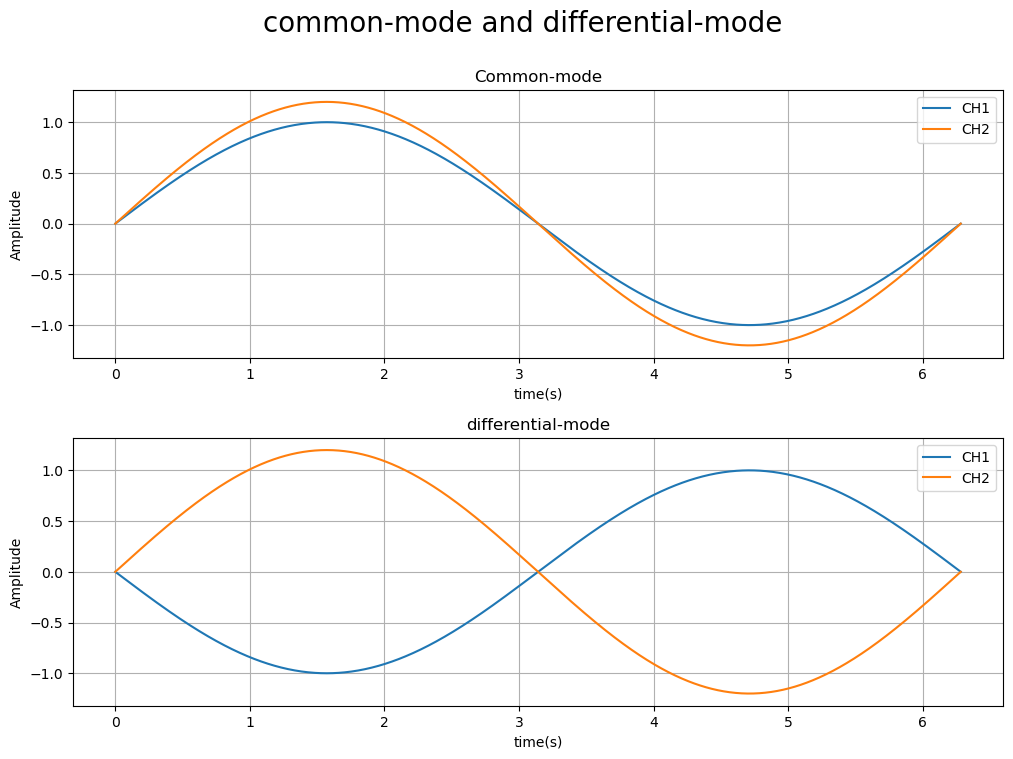
\includegraphics[width=0.5\textwidth]{ET2-1-1.png}
		\caption{共模信号与差模信号示意图}
		\label{fig:ET2-1-1}
	\end{figure}

% 思考题3
\begin{question}
	分析如何实现高的共模抑制比。
\end{question}

	电路的对称性是实现高CMRR的关键因素之一。对称的电路设计可以确保两个输入端的信号在传输过程中受到相同的处理,从而有效抑制共模信号。例如,在差分放大器中,输入级的晶体管或运算放大器的输入端应该尽可能对称,以减少由于不对称引起的共模增益。

	电路中使用的元件(如电阻、电容)应尽可能匹配。元件的不匹配会导致电路不对称,从而降低CMRR。例如,在差分放大器中,输入电阻和反馈电阻的匹配度越高,CMRR越高。

	在信号进入放大器之前,可以使用滤波器来滤除高频噪声,减少共模干扰。此外,信号调理电路也可以帮助提高信号的质量和稳定性。




% \highlight{这一行用来展示高亮。}

% \begin{ubox}{和老婆约会的小曲}
% 	(以下也用于展示更改后的无序列表)
% 	\begin{itemize}
% 		\item 使一颗心免于哀伤;
% 		\item 若我不曾见过太阳。
% 	\end{itemize}
% \end{ubox}

% \highlight[fred]{接下来用于展示代码:}
% \begin{lstlisting}[style=pythonstyle,caption=代码记录示例]
% 	# 示例代码
% 	import matplotlib.pyplot as plt
% 	import numpy as np
	
% 	# Data for plotting
% 	t = np.arange(0.0, 2.0, 0.01)
% 	s = 1 + np.sin(2 * np.pi * t)
	
% 	fig, ax = plt.subplots()
% 	ax.plot(t, s)
	
% 	ax.set(xlabel='time (s)', ylabel='voltage (mV)',
% 	title='About as simple as it gets, folks')
% 	ax.grid()
	
% 	fig.savefig("test.png")
% 	plt.show()
% \end{lstlisting}

